\maketitle

\begin{abstract}
\noindent To construct the mutual solubility curve of a binary two-phase liquid system (for example, 1-butanol/water or methanol/cyclohexane).\thanks{Transcribed from \textcite{nibler14}.}
\end{abstract}

\section{Theory}
\label{sec:theory}

It is sometimes necessary to know the mutual solubilities of liquids in a two-phase system: for example, how much water is dissolved in an organic liquid with which it is in contact, and also the amount of the organic compound that is in the aqueous phase. Although a number of analytical techniques can be used to obtain this information, a procedure that is both conceptually and operationally simple and does not require the removal of liquid samples for analysis (which might change the equilibrium compositions) was described by \textcite{hill1923mutual}. This elegant approach (which Hill called a``thermostatic method'') is based on a volumetric technique and requires knowledge only of the bulk composition of the system, that is, the total mass of each component in the mixture. We assume that the two liquids are in equilibrium in a two-phase system. Thus the phase rule applies.

If you were to combine two pure liquids \(A\) and \(B\), you might find that a two-phase system is formed at a given temperature and pressure. Consider two samples of this binary system that have different bulk quantities of \(A\) and \(B\). Assume that each of the two samples, at the same temperature and pressure, is at equilibrium. See \cref{fig:two_samples}.

\begin{figure}[htb]
	\centering
	\documentclass{standalone}
\usepackage{tikz}

\begin{document}


\hspace*{\fill}
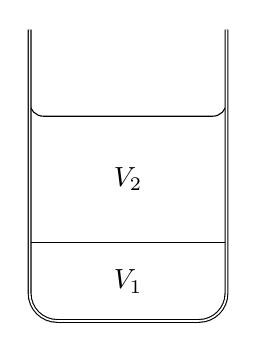
\begin{tikzpicture}
\draw[rounded corners=5] (0,2.8) --
  (0,2.6) --
  (2.5,2.6) --
  (2.5,2.8);
\draw (0,1) -- (2.5,1);
\node at (1.25,1.8) {$V_2$};
\node at (1.25,0.5) {$V_1$};
\draw[double,rounded corners=10] (0,3.7) --
  (0,0)  --
  (2.5,0)  --
  (2.5,3.7);
\end{tikzpicture}
\hspace*{\fill}
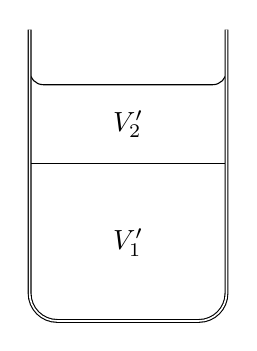
\begin{tikzpicture}
\draw[rounded corners=5] (0,3.2) --
	(0,3.0) --
	(2.5,3.0) --
	(2.5,3.2);
\draw (0,2) -- (2.5,2);	
\node at (1.25,2.5) {$V_2'$};
\node at (1.25,1) {$V_1'$};
\draw[double,rounded corners=10] (0,3.7) --
	(0,0)  --
	(2.5,0)  --
	(2.5,3.7);
\end{tikzpicture}
\hspace*{\fill}


\end{document}
	\caption{Two samples of a two-phase, two-component system containing arbitrary amounts of each component. Both solutions are at the same temperature and pressure.}
	\label{fig:two_samples}	
\end{figure}

If \(m_A\) and \(m_B\) are, respectively, the \emph{bulk masses} of components \(A\) and \(B\) in one sample, and \(m_A^\prime\) and \(m_B^\prime\) are the bulk masses in the other sample, then it follows that
\begin{align}
	m_A &= d_{A1} V_1 + d_{A2} V_2 && \text{and} & m_A^\prime &= d_{A1} V_1^\prime + d_{A2} V_2^\prime
	\label{eq:two_samples_a}\\
	m_B &= d_{B1} V_1 + d_{B2} V_2 && \text{and} & m_B^\prime &= d_{B1} V_1^\prime + d_{B2} V_2^\prime
	\label{eq:two_samples_b}
\end{align}
where \(V_1\) and \(V_2\) are the volumes of the lower phase (higher density) and upper phase (lower density) of one sample, and \(V_1'\) and \(V_2'\) refer to the volumes of the respective phases in the other sample. 
We represent \(d_{A1}\) and \(d_{A2}\) as the equilibrium densities (or mass concentrations) of component \(A\) in phases 1 and 2, respectively. Likewise, \(d_{B1}\) and \(d_{B2}\) are the densities of \(B\) in phases 1 and 2. 
Since the samples are at the same temperature and pressure, the phase rule requires that the equilibrium compositions be the same for both samples (\ie, \(d_{A1} = d_{A1}^\prime\), \(d_{A2} = d_{A2}^\prime\), etc.). 
These equalities are valid assuming that, in the mixed sample, \(A\) and \(B\) can each be treated as a single, chemically independent, component. 

This system can also be described by the phase diagram in \cref{fig:phase_diagram} in which we plot the density against temperature. 
The locus of points on the curve represents phase equilibrium conditions. 
Points inside the curve characterize two phases in coexistence while  those outside the curve indicate the presence of one phase. 
The diagram shows that as \(T\) increases, the density of the lower phase increases while that of the upper phase decreases. 
At some particular temperature, called the critical temperature \((T_c)\), these densities become equal and the two phases coalesce into one.
\begin{marginfigure}
	\documentclass{standalone}
\usepackage{pgfplots,amsmath}
\pgfplotsset{compat=1.18}
\usetikzlibrary{math,arrows.meta}

\begin{document}


\pgfplotsset{
  % height = 0.7\textwidth,
  width = 0.9\textwidth,
  scale only axis,
}

\newcommand{\vertLineFromPoint}[1]{
  \draw[dashed] 
	(#1) -- (#1|-{0,\pgfkeysvalueof{/pgfplots/ymin}})
}

\begin{tikzpicture}
	\begin{axis}[
	clip=true,
	xtick={1},
	xticklabels={$T_c$},
	xmin=-0.1, xmax=1.1, 
	ymin=-1.1, ymax=1.1,
	]
	
	\addplot [mark=none,smooth,thick] coordinates {
				(0.0, 	-1.0)
				(0.19, 	-0.9)
				(0.36, 	-0.8)
				(0.4375, -0.75)
				(0.51, 	-0.7)
				(0.64,	-0.6)
				(0.75,	-0.5)
				(0.84, 	-0.4)
				(0.91, 	-0.3)
				(0.9375, -0.25)
				(0.96, 	-0.2)
				(.99,	-0.1)
				(1.0, 	0.0) 
				(.99,	0.1)
				(0.96, 	0.2)
				(0.9375, 0.25)
				(0.91, 	0.3)
				(0.84, 	0.4)
				(0.75,	0.5)
				(0.64,	0.6)
				(0.51, 	0.7)
				(0.4375, 0.75)
				(0.36, 	0.8)
				(0.19, 	0.9)
				(0, 	1)};	
	
	\draw [dashed] (1.0, 0.0) -- (1.0, -1.1);		
	
	\end{axis}
\end{tikzpicture}

\end{document}

	\caption{Schematic phase diagram of two immiscible liquids. 
	Density is plotted against temperature. 
	The upper and lower portions of the curve represent the densities of the lower and upper phases, respectively.}
	\label{fig:phase_diagram}
\end{marginfigure}

\Cref{eq:two_samples_a,eq:two_samples_b} represent \emph{material balances} that express the equilibrium compositions of the \ch{\(A\)-\(B\)} system as two equations in two unknowns.~\cite{hill1926mutual}
Because the bulk masses (\(m_A\), \(m_A'\), etc.) and the equilibrium volumes (\(V_1\), \(V_1'\), etc.) are \emph{measurable} quantities, the simultaneous solution of \cref{eq:two_samples_a,eq:two_samples_b} allows the four equilibrium concentrations \(d_{A1}\), \(d_{A2}\), \(d_{B1}\), and \(d_{B2}\) to be determined. 
From the two expressions in \cref{eq:two_samples_a} for \(m_A\) and \(m_A'\), we can represent \(d_{A1}\) explicitly using determinants: 
\begin{equation}
	d_{A1} = \frac{
				\begin{vmatrix}
					m_A  & V_2\\
					m_A' & V_2'
				\end{vmatrix}}
				{\begin{vmatrix}
					V_1  & V_2\\
					V_1' & V_2'
				\end{vmatrix}} = \frac{m_A V_2' - m_A' V_2}{V_1 V_2' - V_1' V_2} \,.
	\label{eq:density_one}
\end{equation}
We can substitute this value of \(d_{A1}\) into either of the expressions in \cref{eq:two_samples_a} to find the equilibrium density of component \(A\) in phase 2; using the left-hand one, we get 
\begin{equation}
	d_{A2} = \frac{m_A - d_{A1} V_1}{V_2}
	\label{eq:density_two}
\end{equation}
The identical treatment of the two expressions in \cref{eq:two_samples_b} yields the analogous results for \(d_{B1}\) and \(d_{B2}\). 
More intuitively, we can just replace the \(A\) in \cref{eq:density_one,eq:density_two} by \(B\). 

If we were to study more than two equilibrium samples of \(A\) and \(B\), each exhibiting two phases at the same temperature and pressure, we could determine the densities \(d_{A1}\), \(d_{A2}\), \(d_{B1}\), and \(d_{B2}\) more precisely using a statistical treatment. 
This approach is described in the Appendix. 

The simplicity of the method is very appealing. 
However, it should be clear (and it is mathematical demonstrable) that the approach begins to break down as the mass ration \(m_A/m_B\) in one sample is similar to or approaches the mass ratio in the other sample, \(m_A'/m_B'\). 
In the extreme case where two \emph{identical} samples are considered, no unique information about the system composition can be obtained. 
Moreover, as the ratio of \(m_A'/m_A\) becomes very small (or large), the quality of the information deteriorates because the determined concentrations are sensitive to the error associated with reading the positions of the meniscuses. 
Thus there exists an \emph{optimal} mass ratio that provides maximum precision in the determination of the equilibrium compositions using this methodology (for a given volumetric error). 
Hill was aware of this situation, and in a paper with \textcite{hill1926mutual} presented the analysis of this system optimization. 
We will show just the result here, but if you are curious to see how to obtain the result, see the Appendix. 

\begin{figure}[tb]
	\documentclass{standalone}
\usepackage{tikz}

\begin{document}

\hspace*{\fill}
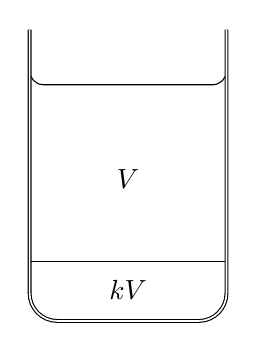
\begin{tikzpicture}
\draw[rounded corners=5] (0,3.2) --
	(0,3.0) --
	(2.5,3.0) --
	(2.5,3.2);
\draw (0,0.75) -- (2.5,0.75);
\node at (1.25,1.8) {$V$};
\node at (1.25,0.4) {$kV$};
\draw[double,rounded corners=10] (0,3.7) --
	(0,0)  --
	(2.5,0)  --
	(2.5,3.7);
\end{tikzpicture}
\hspace*{\fill}
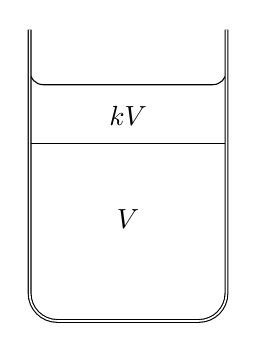
\begin{tikzpicture}
\draw[rounded corners=5] (0,3.2) --
	(0,3.0) --
	(2.5,3.0) --
	(2.5,3.2);
\draw (0,2.25) -- (2.5,2.25);	
\node at (1.25,2.6) {$kV$};
\node at (1.25,1.3) {$V$};
\draw[double,rounded corners=10] (0,3.7) --
	(0,0)  --
	(2.5,0)  --
	(2.5,3.7);
\end{tikzpicture}
\hspace*{\fill}

\end{document}
	\caption{A set of complementary solutions of a two-phase, two-component system at the same temperature and pressure. The volumes of the two phases in the samples are exactly reversed.}
	\label{fig:two_samples_b}
\end{figure}
Consider again two samples of a two-phase liquid system consisting of components \(A\) and \(B\) at the same temperature and pressure. 
These samples are designed so that the volumes are \emph{exactly reversed} for each of the two phases (see \cref{fig:two_samples_b}). 
The ratio of the two phases is denoted by \(k (k>1)\). 
It turns out that the system can be designed to yield the most precise determination of the equilibrium densities  of component \(A\) in the two phases (\(d_{A1}\) and \(d_{A2}\)) if \(k\) has the value 
\begin{equation}
	k_{\text{opt},A} = \frac{d_{A2}}{d_{A1}} \, .
	\label{eq:optimal_ratio_a}
\end{equation}
This ratio of densities (or solubilities, since the two liquids are in equilibrium) is called the \emph{distribution ratio} (or distribution coefficient) of component \(A\) in the two phases and is a thermodynamic quantity because its value depends on equilibrium solubilities. 
Note that \(k\) is presumed to be greater than \num{1}. 
If in reality, however, \(d_{A1} < d_{A_2}\), then the denotation of the phases must simply be reversed---the upper phase in \cref{fig:phase_diagram} is \num{1} and the lower one is \num{2}. 
An analogous result is found for the optimal volume ratio in the complementary solutions for determining the solubility of component \(B\):
\begin{equation}
	k_{\text{opt},B} = \frac{d_{B1}}{d_{B2}} \, .
	\label{eq:optimal_ratio_b}
\end{equation}
In general, these optimal conditions are not the same for the two components because the mutual solubilities of \(A\) and \(B\) are different. 
Nevertheless, \(k_{\text{opt},A}\) and \(k_{\text{opt},B}\) are often close enough that a satisfactory (although not absolute) optimization of the experiment can simultaneously accommodate both components. 
Since the distribution ratio is not known before the experiment is preformed,\sidenote{finding \(d_{A1}\) and \(d_{A2}\) is, after all, the objective of the experiment} a preliminary experiment can be performed to obtain approximate values of the equilibrium compositions. 
From a practical point of view, it is desirable to choose a complementary system in which \(k\) is not too large because in this case relative volumetric errors would become important. 

In this experiment, you will not attempt to seek optimal conditions. 
Rather, you will prepare samples that will provide reasonable accurate results. 
These samples will have complementary volumes (after mixing) that are in a ratio of approximately \(3{:}1\). This means that if the volume ratio of the upper phase to the lower phase in one sample is \(3{:}1\), that ratio for the other sample should be \(1{:}3\).

\section{Safety Precautions}
\label{sec:safety}

\begin{itemize}
	\item Safety glasses or goggles must be worn in the laboratory.
	\item Be particularly careful in removing and manipulating the hot sample cylinders.
	\item Small amounts of organic vapors will be released. 
		Work in an open, well-ventilated laboratory or (preferably) inside a fume hood.
	\item Do not allow the cylinders to build up pressure as they are heated; vent periodically by briefly removing the stoppers.
\end{itemize}

\section{Procedure}
\label{sec:procedure}

\subsection{Required Equipment}
\label{subs:required_equipment}

\begin{itemize}
	\item (2) graduated cylinders (\qty{10}{\mL}) with stoppers
	\item Pasteur pipets
	\item water bath
	\item (1) \qtyrange{0}{100}{\celsius} thermometer
	\item \iupac{cyclohexane} (reagent-grade)
	\item \iupac{methanol} (reagent-grade)
	\item \iupac{1-butanol} (reagent-grade)
	\item distilled water
\end{itemize}

Several different binary liquid systems can be studied using the Hill-Malisoff method. 
The choice depends on such factors as convenience, expense, and ventilation considerations. 
If mutual solubilities are determined at different temperatures, the miscibility diagram of the system can be constructed. 
In this case, it is desirable to study a system that has an upper consolute temperature that is in an experimentally convenient range (that is, less than \qty{100}{\degreeCelsius}). The \emph{upper consolute temperature} is the point above which two liquids are miscible in all proportions (see \cref{fig:phase_diagram}). 

Unfortunately, many of the systems that manifest easily accessible upper consolute temperatures contain a noxious component and must therefore be handled in a fume hood. 
For example, the cyclohexane/aniline system has an upper consolute temperature of \qty{\sim60}{\degreeCelsius}; that of phenol/water is \qty{\sim66}{\degreeCelsius}. Other possible systems are methanol/cyclohexane and \iupac{1-butanol}/water (or other butanol isomers and water). 

In this experiment, you will study the \iupac{1-butanol}/water system or the methanol/cyclohexane system between \qtyrange{0}{\sim70}{\degreeCelsius}. 
Because the upper consolute temperature of the former is \qty{\sim125}{\degreeCelsius}, only a portion of its miscibility curve can be constructed. 
The upper consolute temperature of the latter system, however, is more accessible. 

Prepare two \iupac{1-butanol}/water (or methanol/cyclohexane) samples that manifest two phases at room temperature. 
The volumes of the two phases need not be complementary, but should be distinctly unequal, in a roughly \(3{:}1\) ratio. 
You will determine the densities of the phases for this unoptimized system from \cref{eq:density_one,eq:density_two} (see \cref{fig:two_samples}). 

\begin{enumerate}
	\item Weigh directly into a tared \qty{10}{\mL} graduated cylinder (graduations of \qty{0.1}{\mL}) appropriate amounts (\qty{\pm10}{\mg}) of \iupac{1-butanol} and distilled water (or methanol and cyclohexane) to make a two-phase system with a roughly \(3{:}1\) volume ratio for a total volume of about \qtyrange{6}{7}{\mL}.\sidenote{Remember, meeting a target value is unimportant, but recording the \emph{actual} value is very important.}
	Use a Pasteur pipet to transfer the liquids. 
	Likewise, add the amounts of these components to the other graduated cylinder to make up an approximately complementary two-phase mixture. 
	Label or otherwise identify each cylinder and its stopper. 
	Stopper the cylinders and \emph{gently} invert each several times, venting the cylinder periodically. 
	\item Remove the stoppers and place each of the cylinders in the bath at the lowest temperature (this temperature will be different for the two systems). 
	After a minute, firmly replace each stopper on its respective cylinder. 
	After another minute or so, remove the cylinders one at a time using a test tube holder (or other appropriate device) and carefully invert several times. 
	Replace the cylinder in the bath as quickly as possible. 
	If possible, invert the cylinders directly in the bath. 
	If at this point or in subsequent stages the two phases do not separate cleanly, remove the cylinder and \emph{very gently} tap it on a firm surface. \emph{It is important that the two phases are mixed thoroughly to ensure that phase equilibrium is reached.}\label{stp:bath_one}
	\item Repeat the inversions after \qtyrange{1}{2}{\min}. 
	Wait for a few minutes until the meniscus positions of each samples have become established. 
	Record these positions to the nearest \qty{0.03}{\mL}.\label{stp:meniscus_rec}
	\item Remove the cylinders and place them in the next higher temperature bath (or use an immersion heater to raise the temperature by \qtyrange{5}{10}{\degreeCelsius}). 
	Following the procedures in \cref{stp:bath_one,stp:meniscus_rec}, invert the cylinders and read the meniscus positions after equilibrium is reached. 
	Be sure to vent the cylinder cap briefly to relieve the pressure buildup. 
	\emph{Be careful of escaping vapor.}
	\item Continue this procedure until you reach about \qty{60}{\degreeCelsius}.
	\item For the methanol/cyclohexane system, the upper consolute temperature (or critical solution temperature), \(T_c\), can be determined approximately. 
	Fill a clean cylinder with a mixture (total mass \qtyrange{\sim6}{8}{\g}) that is about \qty{77}{\percent} cyclohexane by mass. 
	Mix thoroughly and place a \qty{2}{\L} beaker that contains sufficient hot water (\qtyrange{\sim55}{60}{\degreeCelsius}) to completely cover the liquid in the cylinder. 
	Invert the cylinder several times; vent periodically to release vapor. 
	The liquid should appear as a homogeneous, one-phase system. 
	Add sufficient quantities of crushed ice to the bath water so that the temperature drops \qtyrange{1}{2}{\degreeCelsius} per minute. 
	Record the temperature at the first sign of a pale blue, hazy appearance to the cooling methanol/cyclohexane mixture. 
	This phenomenon, called \emph{critical opalescence}, appears just above \(T_c\). 
	It is caused by the strong light scattering that accompanies large fluctuations in the density within the sample as the two phases begin to separate. 
	If you overshoot \(T_c\), the system will appear distinctly milky or cloudy. 
	Slowly reheat the system by a few degrees until it homogenizes and then repeat the cooling process. 
	
	The detection of the onset of critical opalescence is best done by having a light source---a bright window, lightbulb, or, better yet, a low-power helium-neon laser---illuminate the sample at \emph{right angles} to the viewing axis (\emph{avoid looking into the laser beam!}). 
\end{enumerate}

\section{Data Analysis}
\label{sec:data_analysis}

\begin{enumerate}
	\item Tabulate the equilibrium volumes of the two phases in each cylinder at the different temperatures studied. 
	\item Using these data, along with the bulk masses of the two components, determine the equilibrium densities \(d_{A1}\), \(d_{A2}\), \(d_{B1}\), and \(d_{B2}\). 
	From this information, obtain the mole fractions of the two components in the two phases at each temperature studied. 
	\item Construct the \(T\)--\(x_A\) phase diagram for the system. 
	It should resemble \cref{fig:sample_t-x_diagram}. 
	For specific guidance, consult your physical chemistry text or your instructor.
	\begin{marginfigure}
		\documentclass{standalone}
\usepackage{pgfplots,amsmath}
\pgfplotsset{compat=1.18}
\usetikzlibrary{math,arrows.meta}

\begin{document}


\pgfplotsset{
  % height = 0.7\textwidth,
  width = 0.9\textwidth,
  scale only axis,
}

\newcommand{\vertLineFromPoint}[1]{
  \draw[dashed] 
	(#1) -- (#1|-{0,\pgfkeysvalueof{/pgfplots/ymin}})
}

\begin{tikzpicture}
	\begin{axis}[
	clip=true,
	xtick={0,1},
	ytick={0.92},
	yticklabels={$T_c$},
	xticklabels={$B$,$A$},
	ylabel={$T$},
	xlabel={$x_a$},
	xmin=0, xmax=1, 
	ymin=0, ymax=1.1,
	]
	
	\addplot [mark=none,smooth,thick] coordinates {
				(0.1, 	0.2)
				(0.2, 	0.4)
				(0.31,	0.6)
				(0.45,	0.8)
				(0.54, 	0.88)
				(0.62,	0.92)
				(0.70,	0.895)
				% (0.67,	0.9)
				(0.75, 	0.8)
				% (0.72, 	0.8)
				(0.81,	0.6)
				(0.86, 	0.4)
				(0.9,	0.2)};	
	\addplot [only marks] coordinates {
				(0.1, 	0.2)
				(0.2, 	0.4)
				(0.31,	0.6)
				(0.45,	0.8)
				(0.75,  0.8)
				(0.81,	0.6)
				(0.86, 	0.4)
				(0.9,	0.2)};	
	
	\draw [dashed] (0, 0.92) -- (0.62,0.92);
	
	\end{axis}
\end{tikzpicture}

\end{document}

		\caption{Schematic \(T\)--\(x_A\) diagram. \(T_c\) is the upper consolute temperature. 
		Each of the four pairs of horizontal circles represents the equilibrium mole fractions of \(A\) in the two phases at the particular temperatures.}
		\label{fig:sample_t-x_diagram}
	\end{marginfigure}
	\item Determine the mutual solubilities of the two components, as well as the distribution (or partition) coefficients at the various temperatures and compare your results with literature values where possible.
\end{enumerate}

\section{Lab Report Guidelines} % (fold)
\label{sec:lab_report_guidelines}

Your lab report should consist of the following parts:
\begin{description}
	\item[Title, Author and Date]
	\item[Introduction] Describe the experiment and expected results in a few sections. 
	\item[Experimental Theory] Reference this document.
	\item[Experimental Procedure] This should be a very brief general outline of the procedure, written out as a paragraph or two. Give the make and model for any major instruments you used, as well as any important settings. The description should be thorough enough that another student can repeat your experiments. This means you must provide explicit volumes, weights, and temperatures. Use the past tense in all of your descriptions. Don't just copy the procedure from the manual, state what work \emph{you} performed. 
	\item[Results and Discussion] This should include an overview of the analyzed data and responses to the questions worked into a natural narrative. 
	Include your data in a \emph{tabular} format, including all the information necessary to repeat your calculations. 
	Include all graphs as figures (with captions). 
	Your graphs should include axes labels (with units). 
	Address the following points in your discussion
	\begin{itemize}
		\item Suppose the distribution coefficient of component \(A\) in a binary system is \num{20}. 
		According to the Hill-Malisoff method, the mass ratio \(m_A/m_B\) for optimal solubility precision is \(20{:}1\). 
		If a \qty{10}{\mL} graduated cylinder is used in the experiment, the smaller volume contained in each tube is less than \qty{0.5}{\mL}. 
		Does this correspond to maximal volumetric precision? 
		How do you decide how to achieve the maximal \emph{overall} experimental accuracy in an experiment such as this?
		\item What other types of analytical methods can be used to determine the compositions of a two-phase liquid system? Discuss approaches that can be used a) without removing samples, and b) by withdrawing small aliquots. 
		\item What is the advantage of applying the Hill-Malisoff method to a binary system contained in a series of \(N\) samples (\(N>2\))?
		\item Can the methodology be extended to a ternary two-phase system?
		Set up the initial equations analogous to \cref{eq:two_samples_a,eq:two_samples_b}. 
		Ternary liquid equilibrium is conveniently studied by ``titrating'' a homogeneous binary phase consisting of components \(A\) and \(B\) with the other component---for example, pure liquid \(A\)---until the mixed ternary system manifests a two-phase appearance. 
		This condition is easily detected as an emulsion.
	\end{itemize}
	\item[References] Include any external material you incorporated into this report (including literature values for physical data). 
	\item[Appendix] At the very end of your report, include examples of any calculations that you did by hand. 
	Include any additional files and code that you used to generate your graphs.
\end{description}
